%\emph{ Tutte le appendici di seguito non provengono dal corso ``Metodi numerici per la fisica'' (``Computational physics laboratory''), ma dal corso del master in ingegneria nucleare ``Physics and numerical models for nuclear reactors'', del prof. Valerio Giusti. }

\chapter{Metodo delle differenze finite}

\subsection*{Introduzione}

Il metodo delle differenze finite è una tecnica numerica utilizzata per approssimare le derivate di una funzione mediante valori della stessa in punti discreti.

Conosciamo bene la definizione di derivata come rapporto incrementale, possiamo quindi usare punti discreti della funzione per svolgere questo rapporto ed approssimare la funzione:

\[
\frac{d\varphi}{dx} =
\lim_{h \to 0}
\frac{\varphi(x+h)-\varphi(x)}{h}
\qquad \text{rapporto incrementale in avanti}
\]

\[
\frac{d\varphi}{dx} =
\lim_{h \to 0}
\frac{\varphi(x)-\varphi(x-h)}{h}
\qquad \text{rapporto incrementale all\'indietro}
\]

\[
\frac{d\varphi}{dx} =
\lim_{h \to 0}
\frac{\varphi(x+h)-\varphi(x-h)}{2\,h}
\qquad \text{rapporto incrementale centrato}
\]

Questo metodo ci dice che considerando il dominio $x\in [0,X]$ e ponendo la \emph{mesh} di N punti, tale che l'intervallo sia $h=X/N$, l'approssimazione della derivata calcolata con punti discreti della funzione può essere calcolata con:

\begin{equation}
	\frac{ d\varphi }{ dx }|_i\,\approx\, \frac{ \varphi_{i+1}-\varphi_i }{h}\ ,\quad 
	\frac{ d\varphi }{ dx }|_i\,\approx\, \frac{ \varphi_{i}-\varphi_{i-1} }{h}\ ,\quad 
	\frac{ d\varphi }{ dx }|_i\,\approx\, \frac{ \varphi_{i+1}-\varphi_{i-1} }{2\,h}\ \ .
\end{equation}

\begin{multicols}{2}
	Nessuna di queste formule è migliore delle altre in ogni occasione, per ogni funzione che si voglia derivare.
	
	Nel caso in figura si vede come il rapporto in avanti è qui il migliore per approssimare la derivata prima.
	
	
	\begin{figure}[H]
		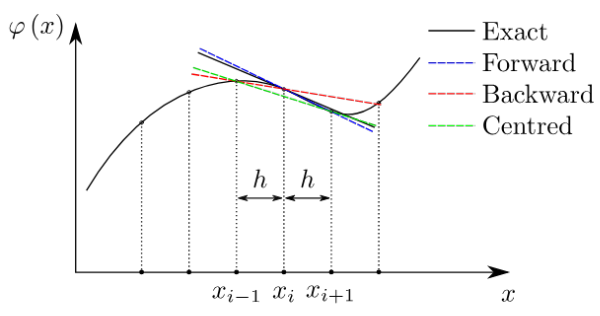
\includegraphics[width=7cm]{img/finitedifferences.png}
		\caption{Prova di applicazione del metodo delle differenze finite al calcolo della derivata prima di una generica funzione polinomiale.}
	\end{figure}
	
\end{multicols}


\subsection*{Accuratezza delle approssimazioni}

Per studiare l'errore utilizziamo lo sviluppo di Taylor.

\[
\varphi(x) =
\varphi(x_0)
+
(x-x_0)\left.\frac{d\varphi}{dx}\right|_{x_0}
+
\frac{(x-x_0)^2}{2}
\left.\frac{d^2\varphi}{dx^2}\right|_{x_0}
+
\frac{(x-x_0)^3}{6}
\left.\frac{d^3\varphi}{dx^3}\right|_{x_0}
+ \dots
\]

Ponendo $x_i = x_0$ otteniamo per $\varphi_{i+1}\,,\ \varphi_{i-1}$:

\[
\varphi_{i+1} =
\varphi_i
+
(x_{i+1}-x_i)
\left.\frac{d\varphi}{dx}\right|_i
+
\frac{(x_{i+1}-x_i)^2}{2}
\left.\frac{d^2\varphi}{dx^2}\right|_i
+
\frac{(x_{i+1}-x_i)^3}{6}
\left.\frac{d^3\varphi}{dx^3}\right|_i
+ \dots
\]

\[
\varphi_{i-1} =
\varphi_i
+
(x_{i-1}-x_i)
\left.\frac{d\varphi}{dx}\right|_i
+
\frac{(x_{i-1}-x_i)^2}{2}
\left.\frac{d^2\varphi}{dx^2}\right|_i
+
\frac{(x_{i-1}-x_i)^3}{6}
\left.\frac{d^3\varphi}{dx^3}\right|_i
+ \dots
\]

Poiché $x_{i+1}-x_i = h$, si ottiene

\begin{equation}\label{i+1 e i-1}
	\begin{aligned}
	\varphi_{i+1} &=
	\varphi_i +
	h \left.\frac{d\varphi}{dx}\right|_i +
	\frac{h^2}{2}\left.\frac{d^2\varphi}{dx^2}\right|_i +
	\frac{h^3}{6}\left.\frac{d^3\varphi}{dx^3}\right|_i + \dots \\
	\varphi_{i-1} &=
	\varphi_i -
	h \left.\frac{d\varphi}{dx}\right|_i +
	\frac{h^2}{2}\left.\frac{d^2\varphi}{dx^2}\right|_i -
	\frac{h^3}{6}\left.\frac{d^3\varphi}{dx^3}\right|_i
	+ \dots
	\end{aligned}
\end{equation}

Da queste espansioni in eq.(\ref{i+1 e i-1}) possiamo riottenere la derivata con metodo forward e backward:

\begin{equation}\label{der}
	\begin{aligned}
	\left.\frac{d\varphi}{dx}\right|_i &=
	\frac{\varphi_{i+1}-\varphi_i}{h} -
	\frac{h}{2}\left.\frac{d^2\varphi}{dx^2}\right|_i -
	\frac{h^2}{6}\left.\frac{d^3\varphi}{dx^3}\right|_i
	+ \dots\ =\\
	& =
	\frac{\varphi_{i+1}-\varphi_i}{h}
	+ O(h)\qquad \text{(\textbf{forward})}\\
	\left.\frac{d\varphi}{dx}\right|_i &=
	\frac{\varphi_i-\varphi_{i-1}}{h}
	\, +\,
	\frac{h}{2}\left.\frac{d^2\varphi}{dx^2}\right|_i
	\, -\,
	\frac{h^2}{6}\left.\frac{d^3\varphi}{dx^3}\right|_i
	+ \dots\ =\\
	& =\ \frac{\varphi_i-\varphi_{i-1}}{h}\, +\, O(h)
	\qquad \text{(\textbf{backward})}
	\end{aligned}	
\end{equation}

Sommando le due espressioni in eq.(\ref{der}) si ottiene

\[
\left.\frac{d\varphi}{dx}\right|_i
\ =\
\frac{\varphi_{i+1}-\varphi_{i-1}}{2h}\,
-\,
\frac{h^2}{6}\,
\left.\frac{d^3\varphi}{dx^3}\right|_i
\,+\,  \dots\ =\
\frac{\varphi_{i+1}-\varphi_{i-1}}{2h}
\,+\,
O(h^2)
\]

Questa formula ha un errore di ordine $h^2$, quindi è più accurata rispetto alle approssimazioni forward e backward che hanno errore $O(h)$.


\subsection*{Approssimazione della derivata seconda}

Sottraendo le due espansioni in eq.(\ref{der}) si ottiene

\[
0\ =\
\frac{\varphi_{i+1}-\varphi_i}{h}
\,-\,
\frac{\varphi_i-\varphi_{i-1}}{h}
\,-\,
h
\left.\frac{d^2\varphi}{dx^2}\right|_i
\,+\,
O(h^3)
\]

da cui segue la formula standard della derivata seconda calcolata con il metodo delle differenze finite:

\begin{equation}
	\left.\frac{d^2\varphi}{dx^2}\right|_i
	\ =\
	\frac{\varphi_{i+1}-2\varphi_i+\varphi_{i-1}}{h^2}
	\,+\,
	O(h^2)
\end{equation}


La stessa espressione può essere ottenuta partendo dalla definizione della derivata seconda, approssimando la derivata prima nei punti intermedi e sostituendo le differenze finite:

\[ \begin{aligned}
\left.\frac{d^2\varphi}{dx^2}\right|_i
\ &=\
\frac{d}{dx}
\left(
\frac{d\varphi}{dx}
\right)_i
\ =\ 
\lim_{h \to 0}
\frac{
	\left.\frac{d\varphi}{dx}\right|_{i+1/2}
	-
	\left.\frac{d\varphi}{dx}\right|_{i-1/2}
}{h}\ =\\
&\approx \ 
\frac{\frac{\varphi_{i+1}-\varphi_i}{h}-\frac{\varphi_i-\varphi_{i-1}}{h}}{h}
\ =\
\frac{\varphi_{i+1}-2\varphi_i+\varphi_{i-1}}{h^2}
\end{aligned} \]



